\subsection{Open Line Wonders: Impedance Insights!}

\begin{tcolorbox}[colback=gray!10, colframe=black, title=E9F11] 

What impedance does a 1/8-wavelength transmission line present to an RF generator when the line is open at the far end?

\begin{enumerate}[label=\Alph*.]
    \item The same as the characteristic impedance of the line
    \item An inductive reactance
    \item \textbf{A capacitive reactance}
    \item Infinite
\end{enumerate} \end{tcolorbox}

\subsubsection{Related Concepts}

To answer this question, one must understand the behavior of transmission lines, particularly the relationship between the length of a transmission line and the impedance it presents to the generator. The key concepts here include:

1. \textbf{Transmission Line Theory:}: A transmission line can transform impedances depending on its length and load. It has a characteristic impedance, denoted as \(Z_0\), which characterizes the line's behavior.

2. \textbf{Wavelength and Impedance Transformation:}: The impedance transformation of a transmission line can be analyzed using the formula:
   \[
   Z_{in} = Z_0 \frac{Z_L + jZ_0 \tan(\beta l)}{Z_0 + jZ_L \tan(\beta l)}
   \]
   Where \(Z_{in}\) is the input impedance, \(Z_L\) is the load impedance, \(l\) is the length of the line, and \(\beta\) is the phase constant related to the wavelength \(\lambda\).

3. \textbf{Open Circuit Condition:}: When the line is open at the far end (\(Z_L = \infty\)), the impedance simplifies.

4. \textbf{1/8 Wavelength Consideration:}: For a transmission line that is \( \frac{1}{8} \) wavelength long (\(l = \frac{\lambda}{8}\)), the phase constant \(\beta\) can be calculated as:
   \[
   \beta = \frac{2\pi}{\lambda}
   \]
   So,
   \[
   \beta l = \frac{2\pi}{\lambda} \cdot \frac{\lambda}{8} = \frac{\pi}{4}
   \]

   The tangent of this angle is:
   \[
   \tan\left(\frac{\pi}{4}\right) = 1
   \]

5. \textbf{Input Impedance Derivation:}: Substituting these values into the impedance transformation formula for an open circuit gives:
   \[
   Z_{in} = Z_0 \frac{Z_L + jZ_0 \tan(\beta l)}{Z_0 + jZ_L \tan(\beta l)} = Z_0 \frac{\infty + jZ_0 \cdot 1}{Z_0 + j\infty \cdot 1}
   \]
   This simplifies to:
   \[
   Z_{in} \to Z_0 \cdot \frac{j}{j} = j \infty \to \text{as } Z_L \text{ becomes infinite}
   \]

6. \textbf{Final Impedance Result:}: Therefore, we need to evaluate the \( \frac{1}{8} \)-wavelength effect, where the transmission line presents a capacitive impedance back to the RF generator.

\subsubsection{Calculation Summary}

The calculations show that the 1/8-wavelength open line behaves as a capacitive reactance rather than an inductive reactance or an infinite impedance. 

\subsubsection{Diagram}

\begin{center}
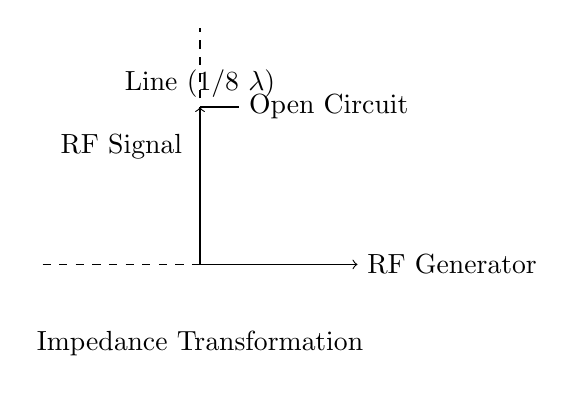
\begin{tikzpicture}
    \draw[->] (0,0) -- (0,2) node[above] {Line (1/8 $\lambda$)};
    \draw[->] (0,0) -- (2,0) node[right] {RF Generator};
    \draw (0,2) -- (0.5,2) node[right] {Open Circuit};
    \draw[dashed] (-2,0) -- (2,0);
    \draw[dashed] (0,0) -- (0,3);
    \node at (-1,1.5) {RF Signal};
    \node at (0,-1) {Impedance Transformation};
\end{tikzpicture}
\end{center}
